\section{Assignment 1 (50 Points)}
\label{sec:assignment1}

\subsection*{Questions}
\begin{enumerate}[label=\alph*.]
    \item Compute your friend's $d'$ in a working memory task. You may read out the words, use PowerPoint slides, or program them (e.g., \texttt{Matlab}).
    
    \item Does $d'$ vary with set size? Plot $d'$ versus set size --- this is called a \textit{psychophysical function}.
    
    \item Does bias vary with set size? Interpret your findings from (a) and (b). \hfill (30 points)
    
    \item Construct an ROC curve and show how it relates to $d'$. \textit{Hint:} How do you ensure that your subject varies her/his criteria? \hfill (20 points)
\end{enumerate}

\noindent\textbf{Useful formulas:}
\begin{align}
    d' &= \Phi^{-1}(H) - \Phi^{-1}(F)\\
    c &= -\Phi^{-1}(F)\\
    b &= -\frac{\Phi^{-1}(H) + \Phi^{-1}(F)}{2}
\end{align}

\begin{figure}[h!]
    \centering
    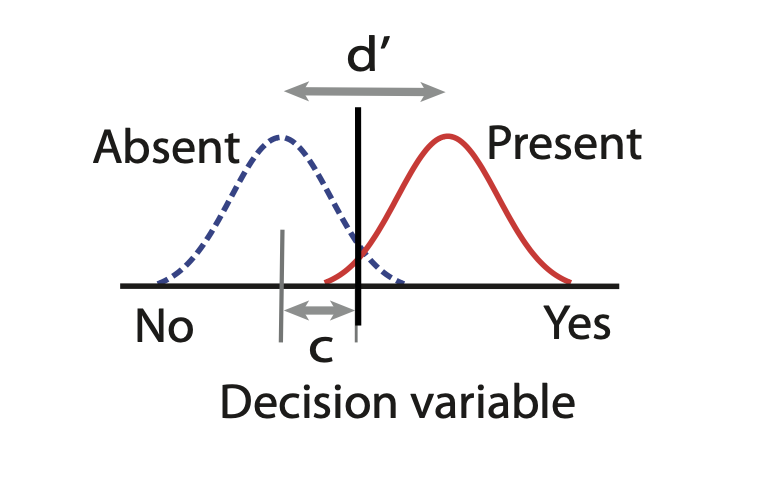
\includegraphics[width=0.8\textwidth]{figures/assignment1.png}
    \caption{Example of an assignment figure.}
\end{figure}

\newpage
\subsection*{Answers}

\noindent\textbf{(a) Computation of $d'$:}

An \texttt{HTML}-based application was developed to conduct the experiment. The program automatically saved the results as a \texttt{.csv} file for further analysis and computation. A pool of approximately 150 words was used (listed in Section~\ref{sec:appendix}), from which a random subset was selected for each trial. The subject was instructed to memorize the displayed words for 5 seconds in each trial. Afterward, a test word was presented, and the subject indicated whether it was part of the original set and rated her confidence in the response on a 5-point scale (1 = Guessing, 2 = Unsure, 3 = Moderate, 4 = Confident, 5 = Certain).

The complete code and recorded results are provided in the Appendix. Informed consent was obtained from the subject (Dr.~Gnaani, MBBS, MMST). The experiment was conducted with set sizes ranging from 2 to 15 words, with 15 trials per set, resulting in a total of 165 observations. The obtained dataset is shown below.

\begin{table}[H]
    \centering
    \caption{Experimental results showing Signal Detection Theory parameters ($d'$, criterion $c$, bias $b$, and AUC) derived from participant responses.}
    \label{tab:dataset}
    \small
    \begin{tabular}{lcccccccccc}
        \toprule
        \textbf{Set} & \textbf{n\_sig} & \textbf{n\_noise} & \textbf{Hit} & \textbf{FA} & \textbf{zH} & \textbf{zF} & \textbf{$d'$} & \textbf{$c$} & \textbf{$b$} & \textbf{AUC} \\
        \textbf{Size} & & & \textbf{Rate} & \textbf{Rate} & & & & & & \\
        \midrule
        2  & 9 & 6  & 0.94 & 0.08 & 1.59 & $-1.38$ & 2.98 & $-0.11$ & $-0.11$ & 0.98 \\
        3  & 5 & 10 & 0.90 & 0.05 & 1.28 & $-1.64$ & 2.93 & 0.18  & 0.18  & 0.98 \\
        4  & 5 & 10 & 0.90 & 0.05 & 1.28 & $-1.64$ & 2.93 & 0.18  & 0.18  & 0.98 \\
        5  & 5 & 10 & 0.80 & 0.05 & 0.84 & $-1.64$ & 2.49 & 0.40  & 0.40  & 0.96 \\
        6  & 8 & 7  & 0.94 & 0.07 & 1.53 & $-1.47$ & 3.00 & $-0.03$ & $-0.03$ & 0.98 \\
        7  & 9 & 7  & 0.94 & 0.07 & 1.59 & $-1.47$ & 3.06 & $-0.06$ & $-0.06$ & 0.98 \\
        8  & 8 & 6  & 0.94 & 0.08 & 1.53 & $-1.38$ & 2.92 & $-0.08$ & $-0.08$ & 0.98 \\
        9  & 3 & 12 & 0.83 & 0.17 & 0.97 & $-0.97$ & 1.93 & 0.00  & 0.00  & 0.91 \\
        10 & 8 & 7  & 0.88 & 0.14 & 1.15 & $-1.07$ & 2.22 & $-0.04$ & $-0.04$ & 0.94 \\
        12 & 5 & 10 & 0.90 & 0.30 & 1.28 & $-0.52$ & 1.81 & $-0.38$ & $-0.38$ & 0.90 \\
        15 & 7 & 8  & 0.86 & 0.63 & 1.07 & 0.32  & 0.75 & $-0.69$ & $-0.69$ & 0.70 \\
        \bottomrule
    \end{tabular}
\end{table}

\noindent\textbf{(b) Variation of $d'$ with set size:}

Yes, $d'$ (sensitivity) decreased monotonically with set size. The subject exhibited higher discriminability when the memory load was low. As the set size increased, both internal noise and cognitive load rose, leading to a progressive decline in perceptual sensitivity ($d'$). The psychophysical function shows that $d'$ remained relatively high ($\sim$3.0) for smaller set sizes (2--7) but declined sharply from set size 9 ($\approx$2.0), reaching about 0.75 at the largest set size (15).

\begin{figure}[H]
    \centering
    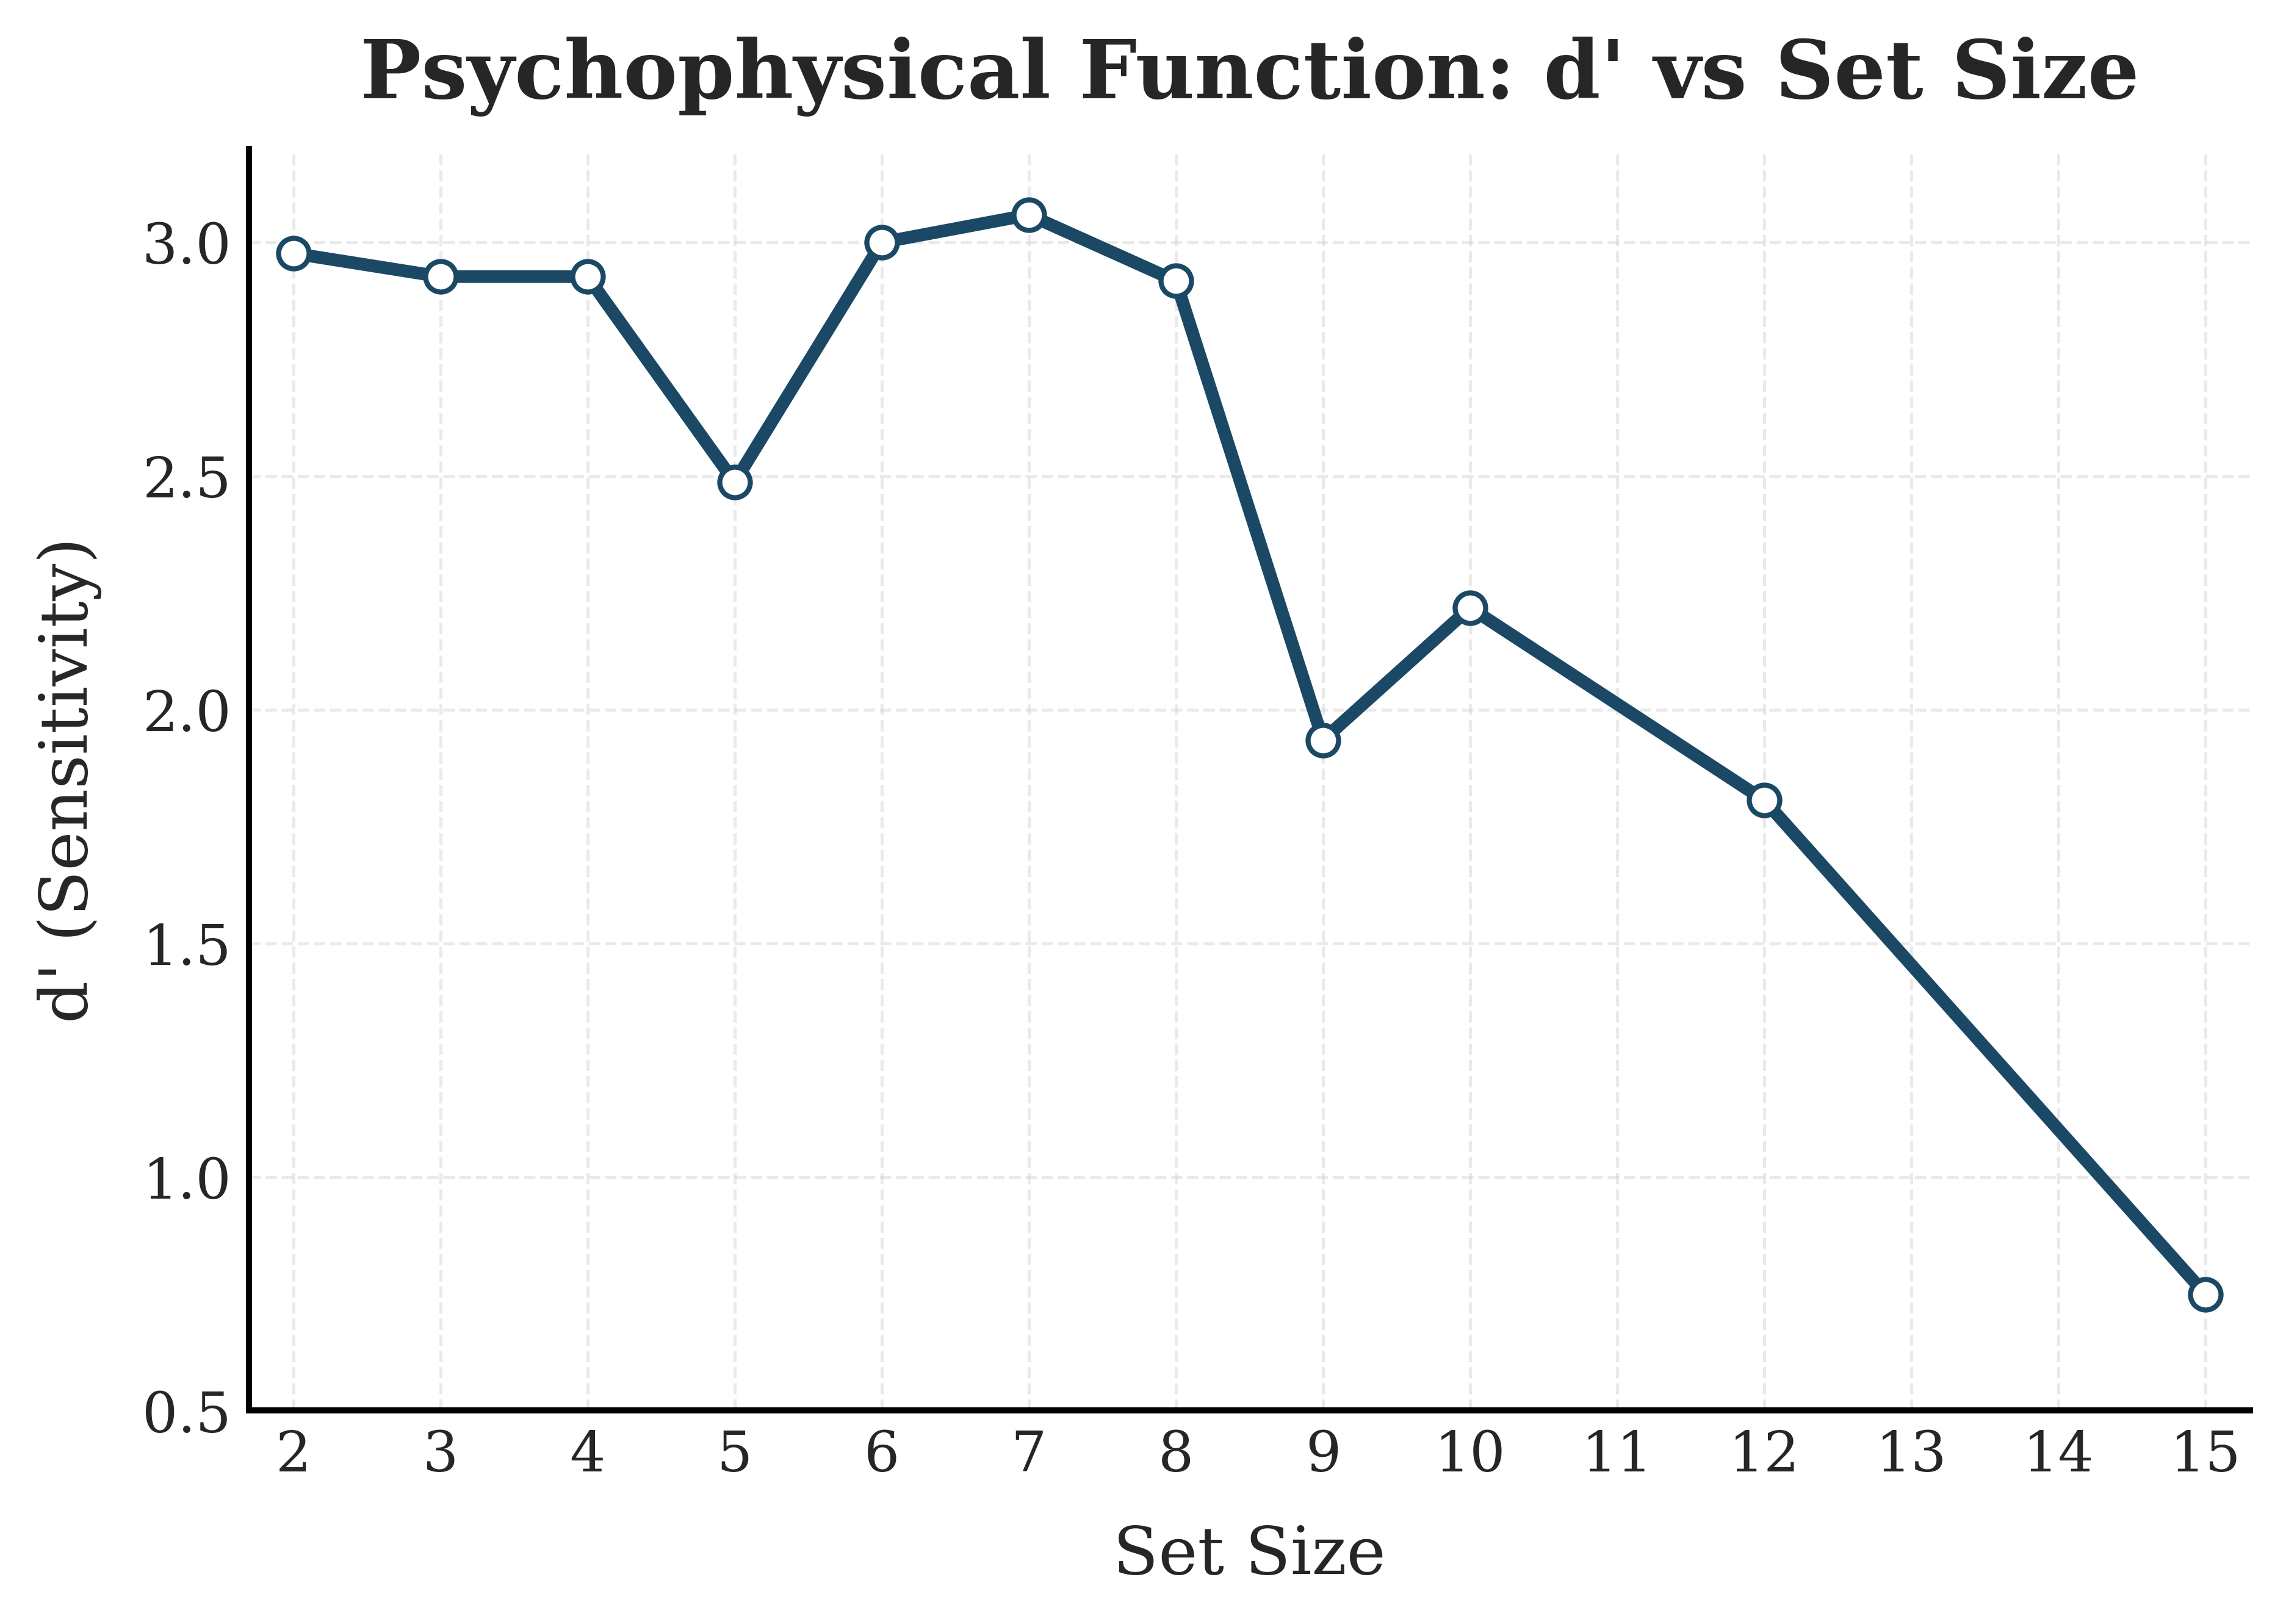
\includegraphics[width=0.75\textwidth]{figures/plot0.png}
    \caption{Psychophysical function showing the variation of sensitivity ($d'$) with set size. As the number of words in the memory set increases, sensitivity ($d'$) decreases, indicating reduced discriminability.}
    \label{fig:dprime_vs_setsize}
\end{figure}

\noindent\textbf{(c) Bias variation with set size:}

Yes, bias varies with set size. My subject showed variable bias patterns as the task difficulty changed. The bias function (criterion $c$) shows a conservative bias (positive values) for smaller set sizes (2--5), with a peak at set size 5 ($c \approx 0.4$). This indicates participants were more likely to respond ``No.'' The criterion then drops and fluctuates around zero for moderate set sizes (6--10), indicating a relatively neutral response strategy. However, at larger set sizes (12--15), criterion $c$ becomes increasingly negative, meaning participants tend to respond ``Yes'' more often, adopting a liberal bias as the task becomes harder.

\begin{figure}[H]
    \centering
    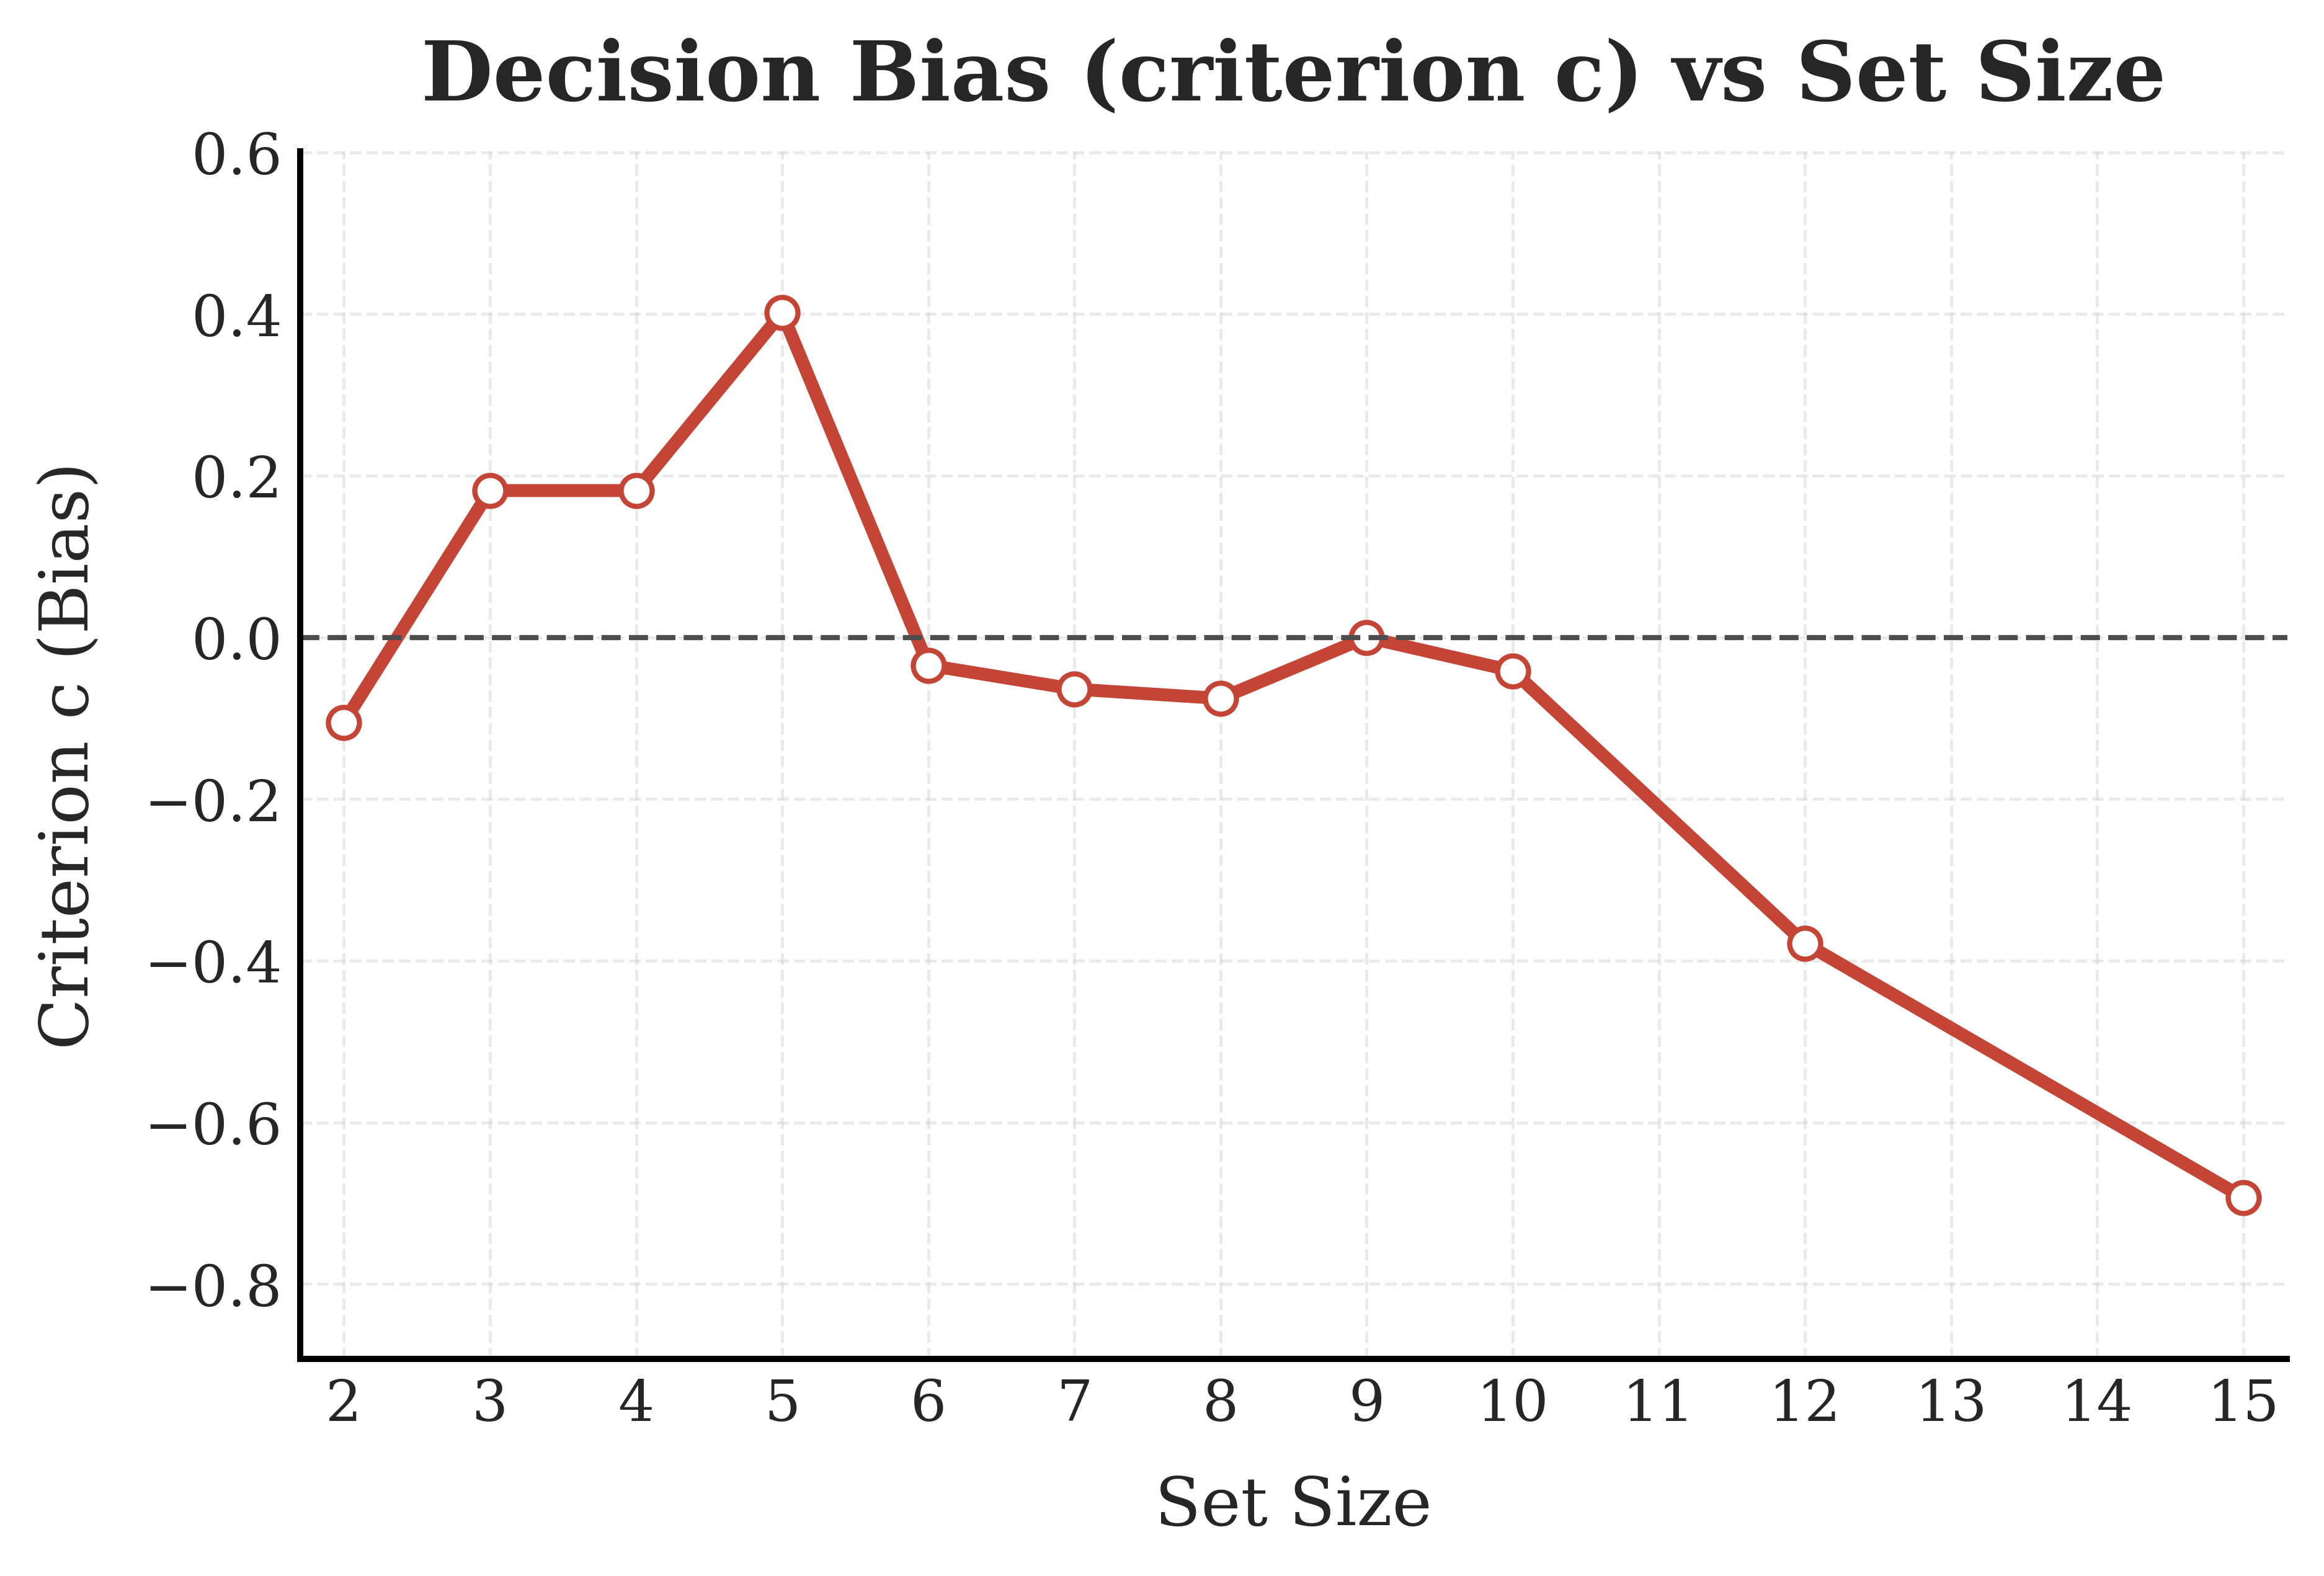
\includegraphics[width=0.75\textwidth]{figures/plot1.png}
    \caption{Variation of criterion $c$ with set size. Positive values indicate conservative bias, negative values indicate liberal bias. The criterion shifts from conservative to liberal as set size increases, with the dashed line marking neutral bias ($c = 0$).}
    \label{fig:criterion_vs_setsize}
\end{figure}

\noindent\textbf{(d) ROC curve and relation to $d'$:}

To construct \texttt{ROC curves} with varying criteria, confidence ratings were collected from the subject on each trial. These ratings allowed me to plot multiple hit rate--false alarm rate pairs by treating each confidence level as a different decision threshold.

\begin{figure}[H]
    \centering
    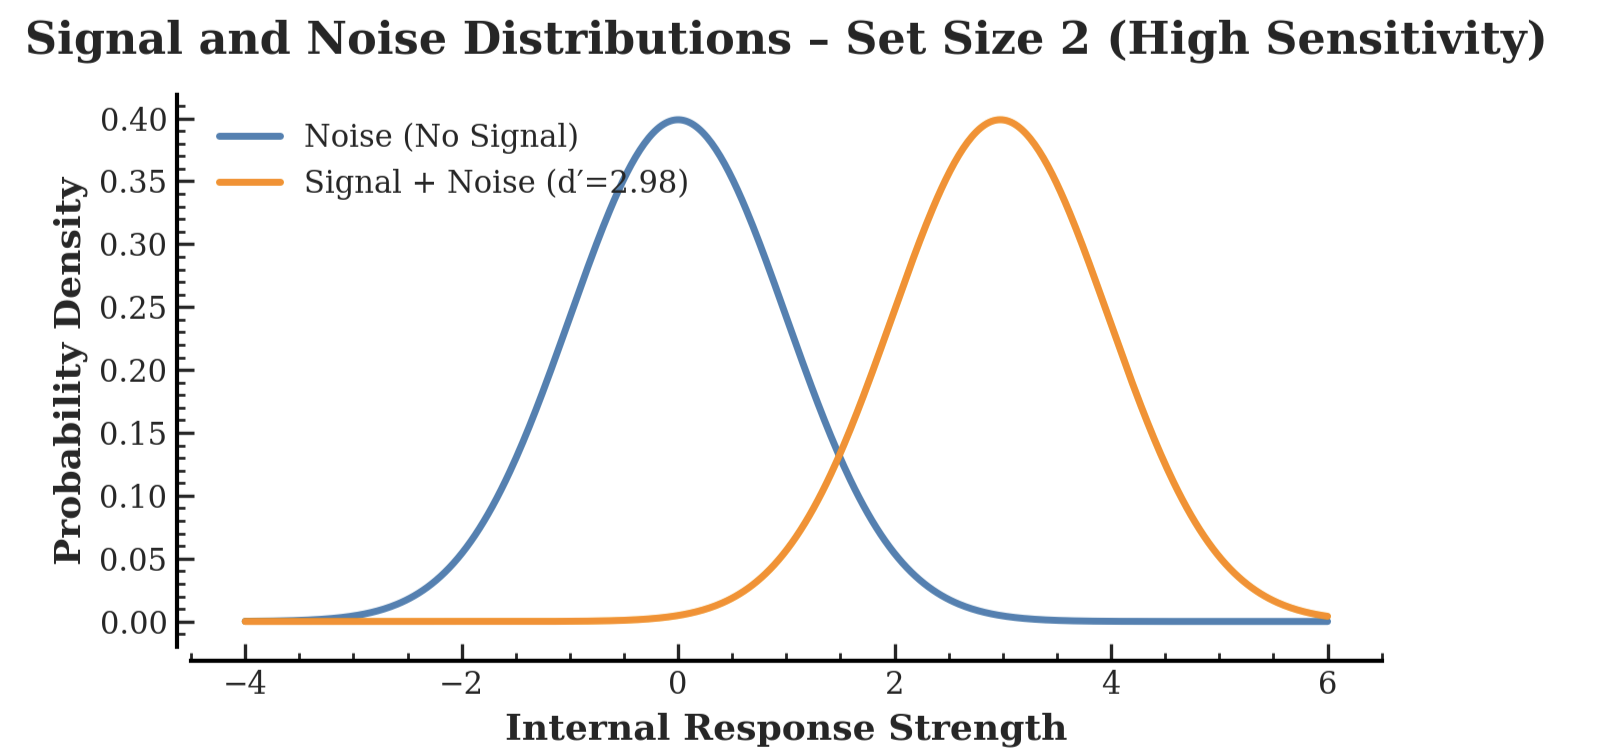
\includegraphics[width=0.75\textwidth]{figures/n_S_S2.png}
    \caption{Signal and noise distributions for Set Size 2 (high sensitivity). The large separation between distributions ($d' \approx 2.98$) indicates strong discriminability.}
    \label{fig:sig_noise_set2}
\end{figure}

For small set sizes, the noise and signal-plus-noise distributions show clear separation. My subject could easily distinguish signal-present trials, resulting in a more bowed ROC curve with high area under the curve (AUC).

\begin{figure}[H]
    \centering
    \includegraphics[width=0.75\textwidth]{figures/n_S_S15.png}
    \caption{Signal and noise distributions for Set Size 15 (low sensitivity). The substantial overlap between distributions ($d' \approx 0.75$) indicates reduced discriminability.}
    \label{fig:sig_noise_set15}
\end{figure}

At larger set sizes, the overlap between the two distributions increases significantly. My subject's internal responses for signal and noise trials became less distinct, producing a flatter ROC curve closer to the chance diagonal.

\begin{figure}[H]
    \centering
    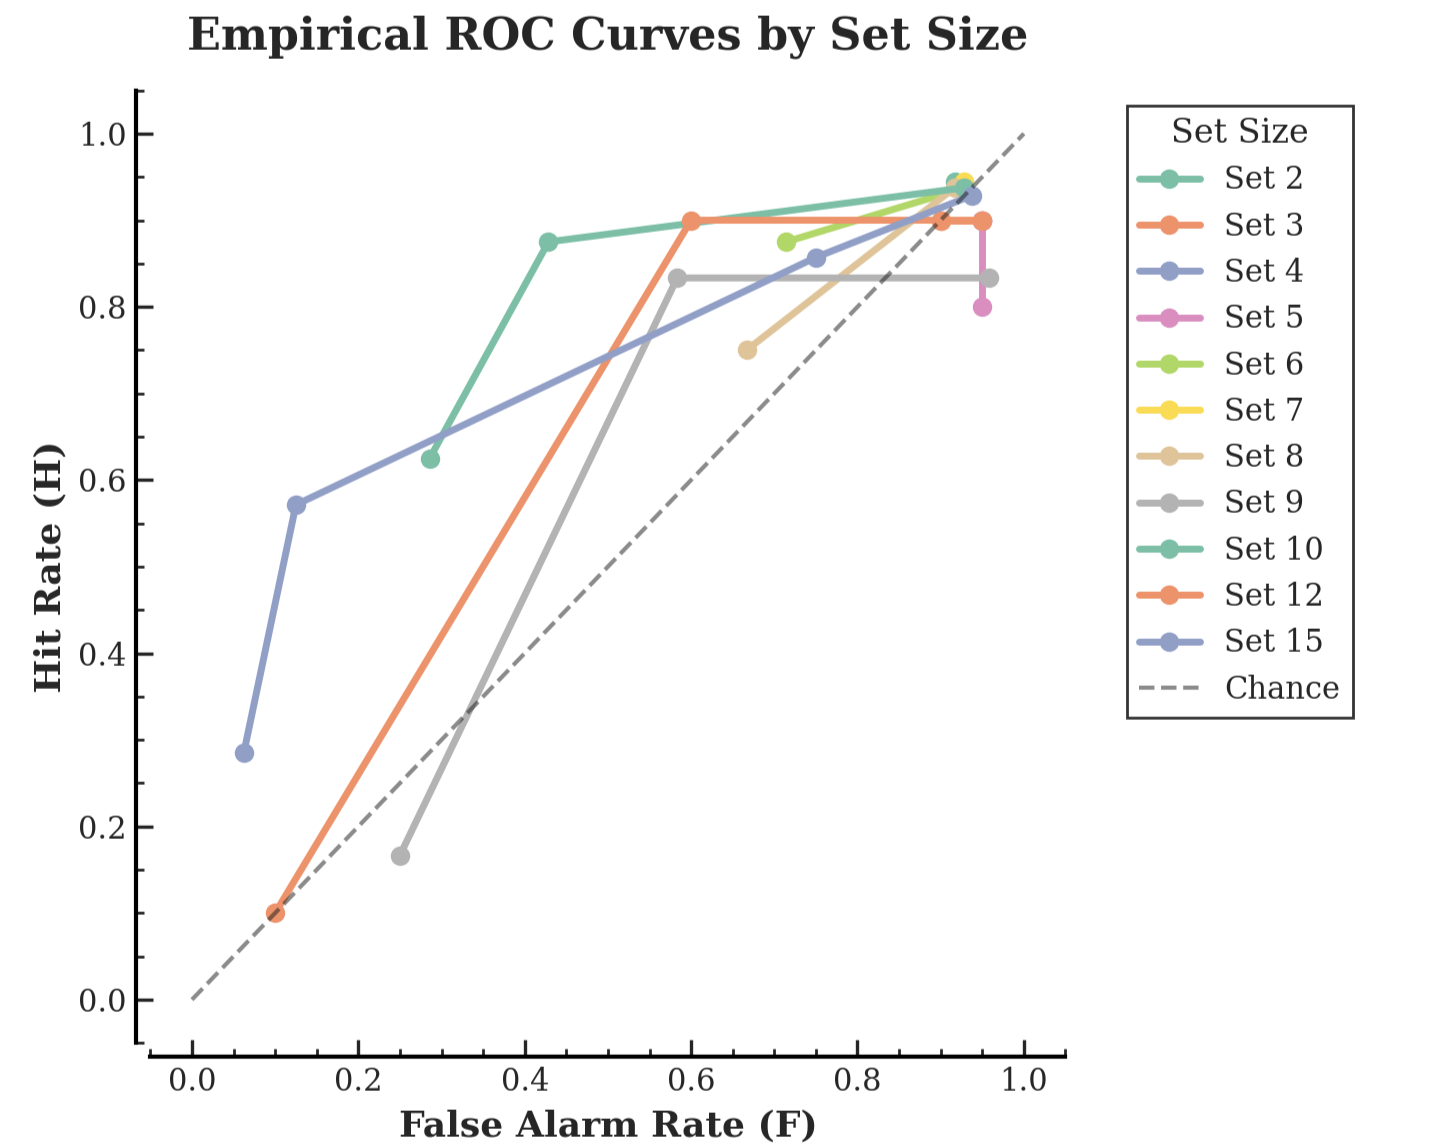
\includegraphics[width=0.78\textwidth]{figures/ROC.png}
    \caption{Empirical ROC curves for each set size. Each point represents a different confidence threshold. As set size increases, ROC curves become less bowed and approach the diagonal, indicating reduced sensitivity.}
    \label{fig:empirical_roc}
\end{figure}

The discrete, step-wise shape of the empirical ROC curves arises because each point corresponds to one of the subject's five confidence thresholds. This pattern is typical for behavioral data collected with discrete confidence ratings (Macmillan \& Creelman, 2005).

\begin{figure}[H]
    \centering
    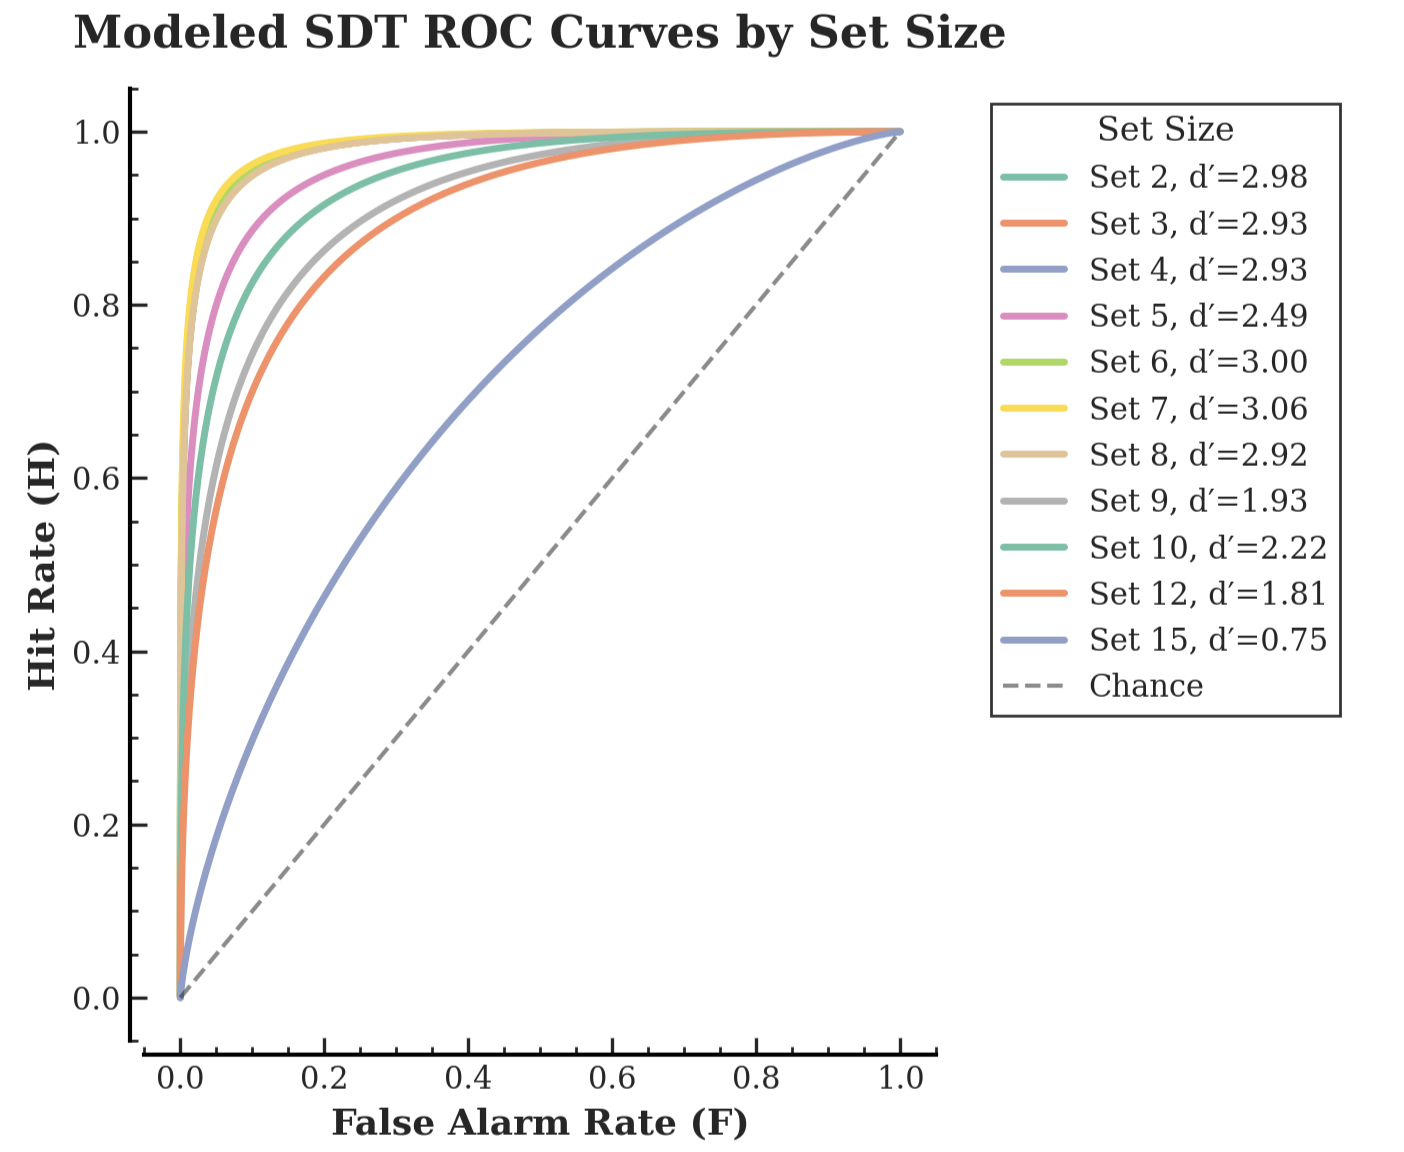
\includegraphics[width=0.78\textwidth]{figures/ModelSDTROC.png}
    \caption{Modeled ROC curves generated using equal-variance SDT formulation for each set size. Larger $d'$ values produce more bowed curves (greater discriminability), while smaller $d'$ values produce flatter curves closer to chance.}
    \label{fig:modeled_roc}
\end{figure}

The relationship between ROC curves and $d'$ is clearly demonstrated: as sensitivity decreases with increasing set size, the ROC curves progressively flatten, moving from highly bowed curves (high $d'$) toward the diagonal line representing chance performance (low $d'$). This direct correspondence validates the Signal Detection Theory framework for understanding working memory performance.